\chapter{Figma Design}

\section{Description}
% Briefly decribe the idea of the app
The main idea for this application is to provide a hub for people to find travel destinations. It should help find the points-of-interest (or events) in the surrounding area of the user.
Users can browse a list of destinations using filters to specify categories such as type (e.g., place, event, ...) and save items to their favourites in their account. 


\section{Design Philosophy}

We use a consistent design strategy to provide an easy to understand experience to the user. The screen is divided into different content sections. At the bottom we place a menu-bar to facilitate navigation to the main screens of our application, namely \textsl{Home}, \textsl{Account} and \textsl{FAQ}. This bar will always be on visible throughout all pages/screens of our app.

The top row of the screen is taken by a dynamic content header. More specifically, it will show a descriptive text depending on the context. On the home screen, it will show the content of the search bar, in the details screen it will show the title text of the item that is shown. In case of \textsl{Account}, \textsl{Sign-up} and \textsl{Log-in} it will simply tell the page name.

The majority of the screen will be comprised of a centre content panel. It will show them main content of each page. More details on this content in the next section.

\section{Design Prototype}

\subsection*{Home}
On start-up the user will be presented with the our main screen. A design-sketch can be seen in Fig. \ref{fig:homepage}. This screen features a search bar to find items by name, or query a specific key attribute (e.g., beach, church, monument, ...). Filters can be set through filter options in below the search bar.
The main content of \textsl{Home} page, consists of previews of content items corresponding to the filters set by the user. Each item shows a big thumbnail image, the title, rating and whether the item is already in the users favourite list. If available, the price attribute is shown as well.

\subsection*{Details}
On \textsl{Details} a detailed description, along with picture(s), a rating score and eventual pricing is shown. Below we show user ratings to the item (if exist).
We indicate whether the item is a \textit{favourite}, in the same way as on the home page, by a little heart symbol in the to right corner of the item picture. The design can be found in Fig. \ref{fig:details}.

\begin{figure}
	\centering
	\begin{subfigure}[T]{0.4\linewidth}
		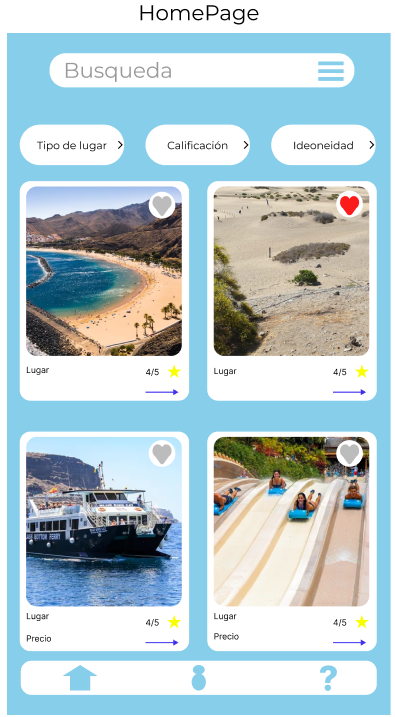
\includegraphics[width=\linewidth]{figures/homepage.png}
		\caption{Design for the home page of our app}
		\label{fig:homepage}
	\end{subfigure}
	\hfill
	\begin{subfigure}[T]{0.4\linewidth}
		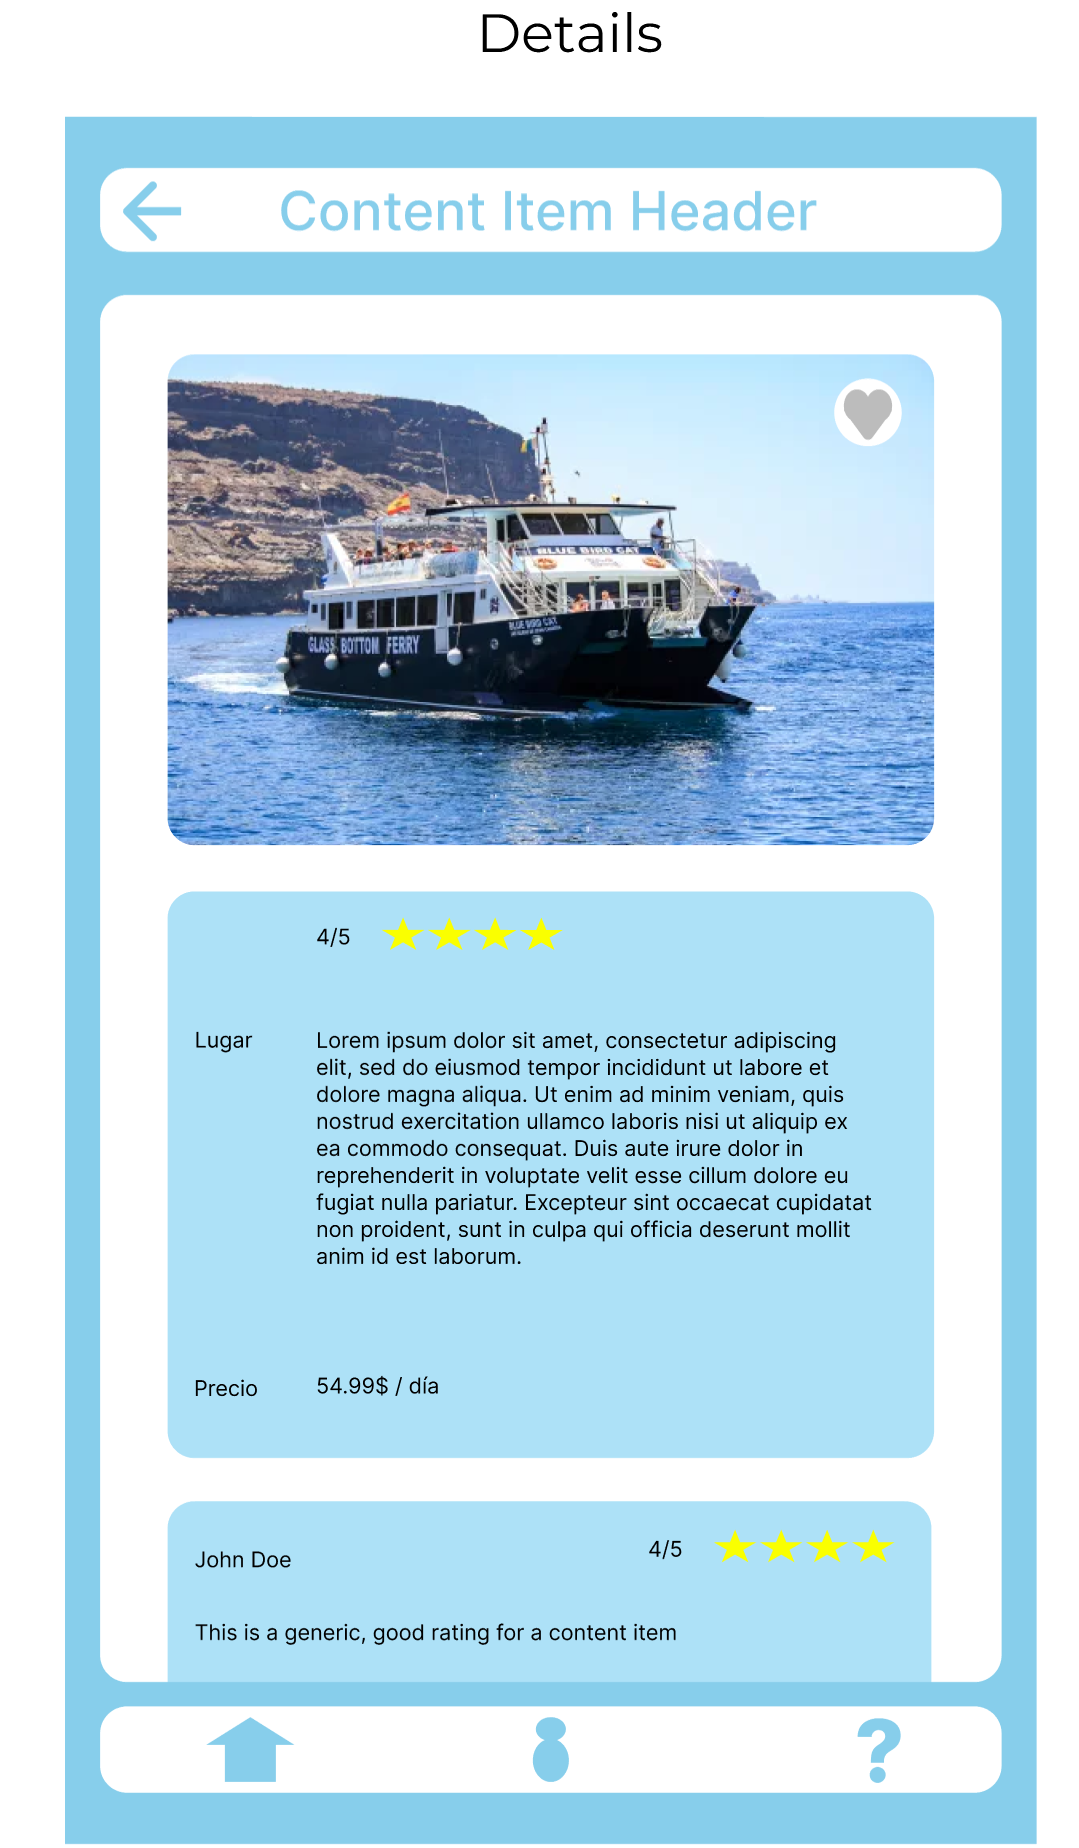
\includegraphics[width=\linewidth]{figures/details.png}
		\caption{Design for the content item details page of our app}
		\label{fig:details}
	\end{subfigure}
\end{figure}

\subsection*{FAQ}
This page serves as a general information and support page to the user. It will feature guidelines, \textit{"How to use the service"} information and of course the frequently asked questions users may have. See the design proposal in Fig. \ref{fig:FAQ}.


\subsection*{Account}
The account page shows the users information, profile picture and name. A user may modify personal information such as bio-text, picture or (shown) real-name. The username may not be changeable since it would serve as a UID. See the design in Fig. \ref{fig:account}

\begin{figure}
	\centering
	\begin{subfigure}[T]{0.4\linewidth}
		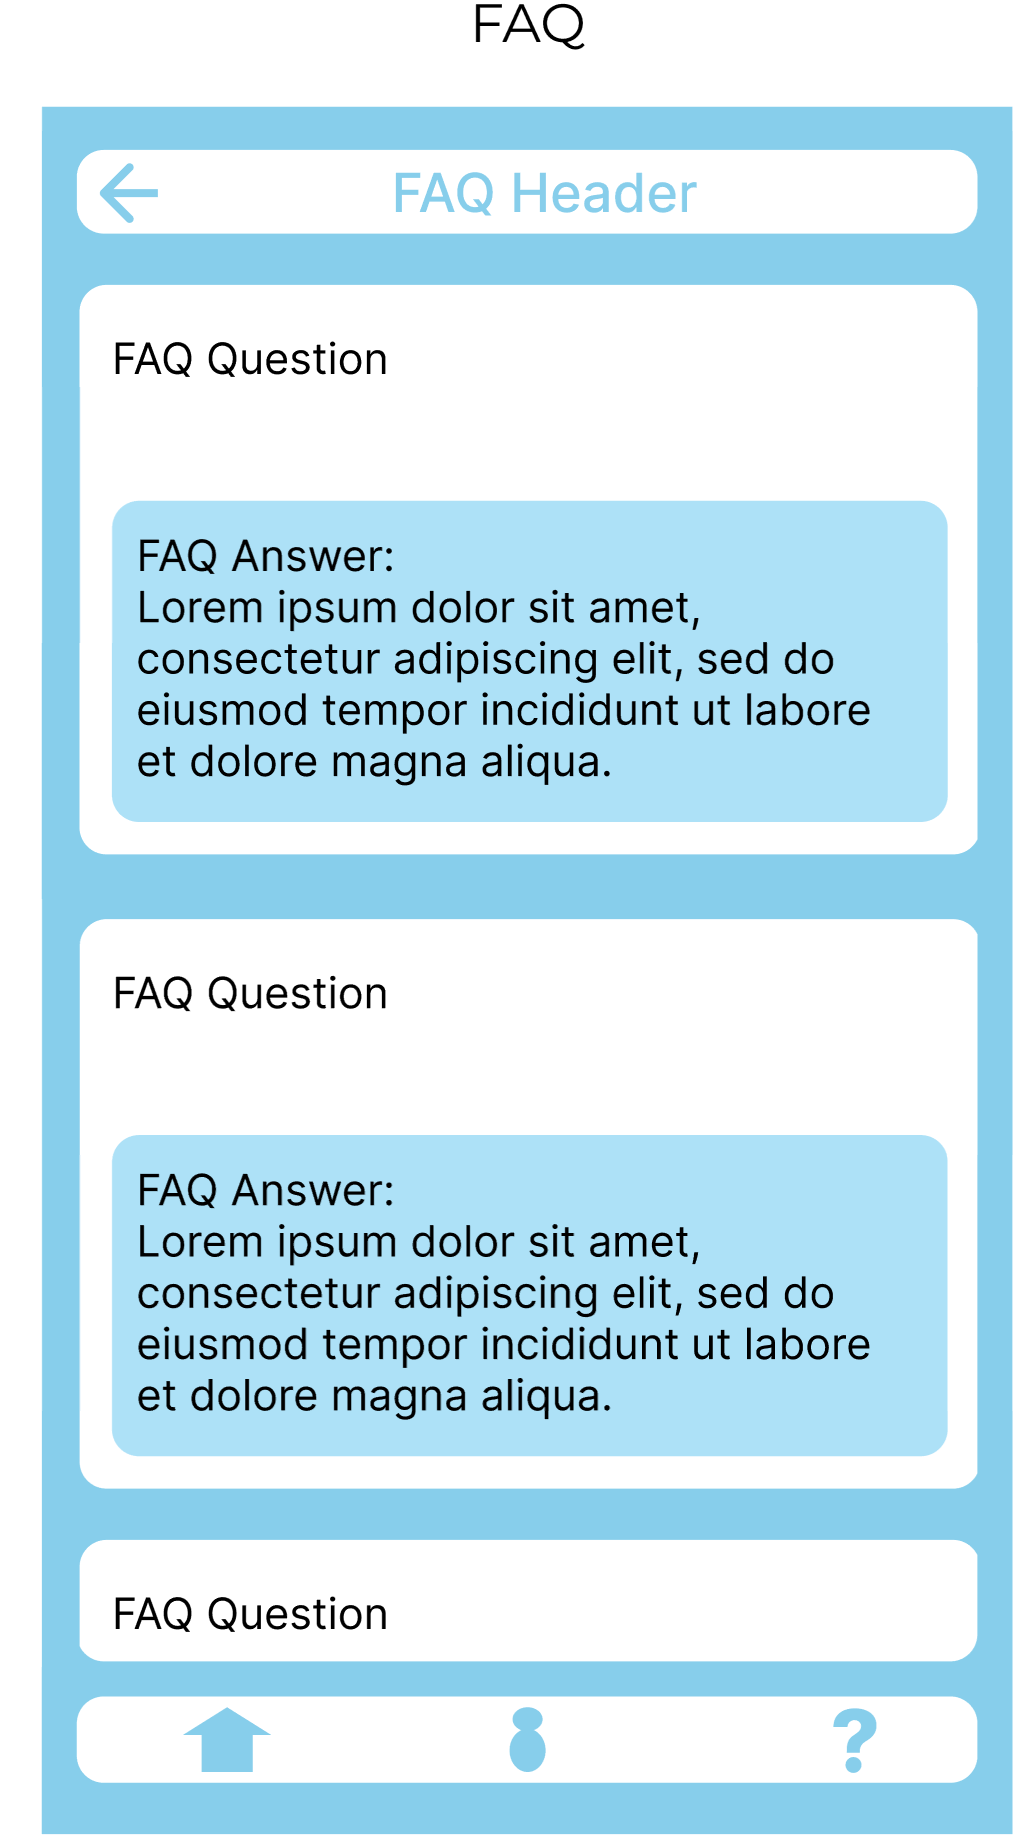
\includegraphics[width=\linewidth]{figures/FAQ.png}
		\caption{Design for the FAQ page of our app}
		\label{fig:FAQ}
	\end{subfigure}
	\hfill
	\begin{subfigure}[T]{0.4\linewidth}
		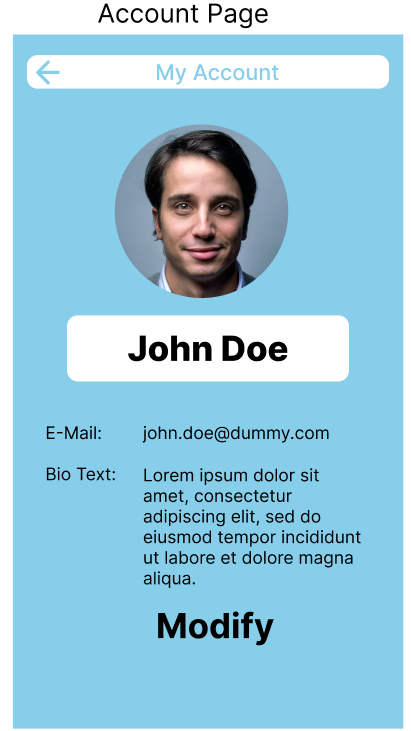
\includegraphics[width=\linewidth]{figures/account.png}
		\caption{Design for the account page of our app}
		\label{fig:account}
	\end{subfigure}
\end{figure}

\subsection*{Sign-Up}
This page is shown if a user tries to log in without an account and need to create one. It is comprised of a simple form to enter personal information. The personal information may be subject to change throughout the development process. The first draft can be seen in Fig. \ref{fig:sign_in}.

\subsection*{Log-In}

The \textsl{Log-In} screen is shown to the user when ever the user is not already logged in and tries to perform an action such as rating, favour-ize an item or see the personal account (hence actions that require to be logged in).
It features a form to enter log-in credentials. See the design for the page in Fig. \ref{fig:log_in}.


\begin{figure}
	\centering
	\begin{subfigure}[T]{0.4\linewidth}
		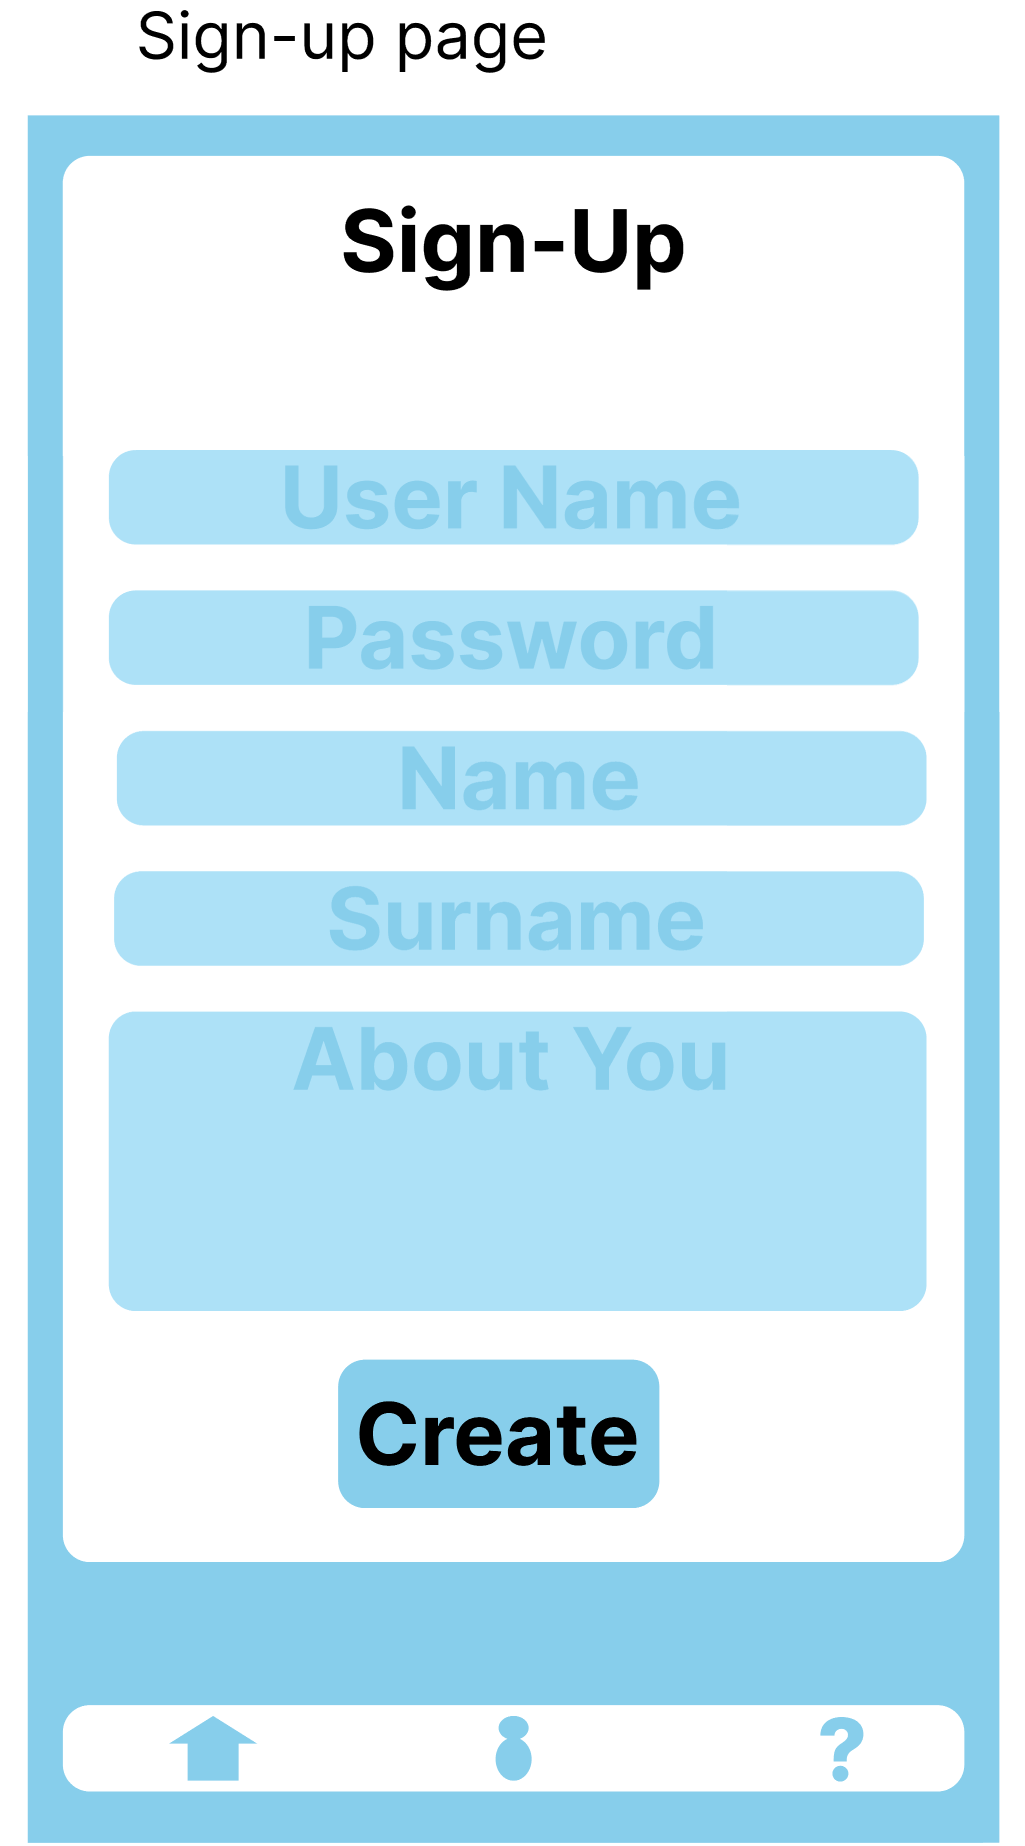
\includegraphics[width=\linewidth]{figures/sign_up.png}
		\caption{Design for the sign-up page of our app}
		\label{fig:sign_in}
	\end{subfigure}
	\hfill
	\begin{subfigure}[T]{0.4\linewidth}
		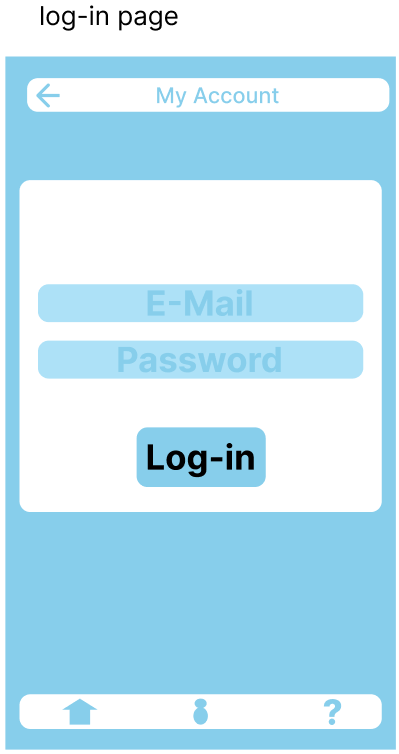
\includegraphics[width=\linewidth]{figures/log_in.png}
		\caption{Design for the log-in page of our app}
		\label{fig:log_in}
	\end{subfigure}
\end{figure}
